\documentclass[tikz,border=5pt]{standalone}
\usepackage{tikz}
\usetikzlibrary{positioning,calc}

\begin{document}
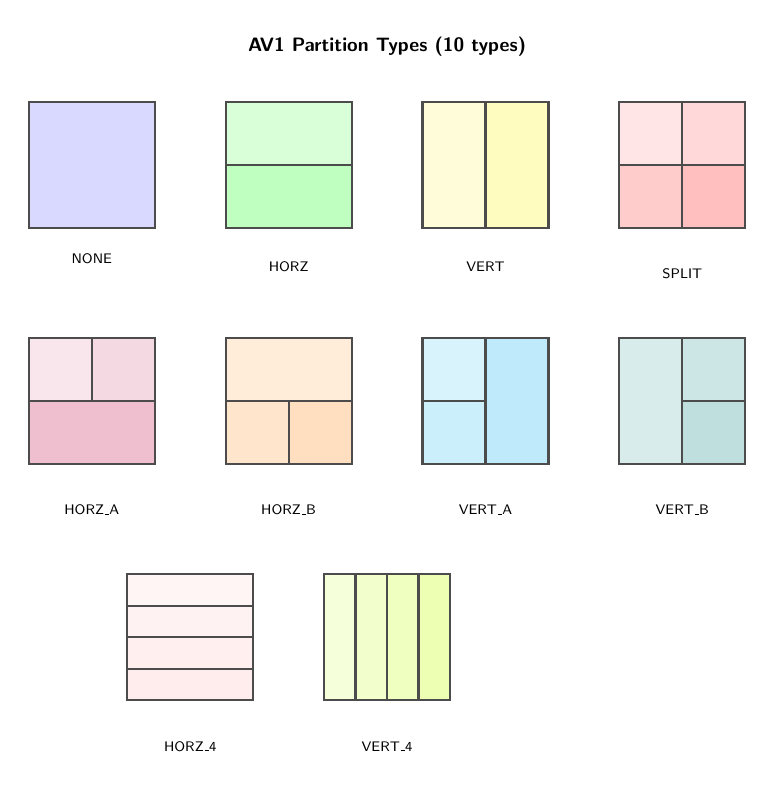
\begin{tikzpicture}[
    block/.style={draw=black!70, thick, minimum width=1.6cm, minimum height=1.6cm},
    halfh/.style={draw=black!70, thick, minimum width=1.6cm, minimum height=0.8cm},
    halfw/.style={draw=black!70, thick, minimum width=0.8cm, minimum height=1.6cm},
    quarter/.style={draw=black!70, thick, minimum width=0.8cm, minimum height=0.8cm},
    stripe/.style={draw=black!70, thick, minimum width=1.6cm, minimum height=0.4cm},
    vstripe/.style={draw=black!70, thick, minimum width=0.4cm, minimum height=1.6cm},
    label/.style={font=\tiny\sffamily, below=0.2cm},
    title/.style={font=\scriptsize\sffamily\bfseries}
]

% Row 1: NONE, HORZ, VERT, SPLIT
\begin{scope}[shift={(0,0)}]
    \node[block, fill=blue!15] (none) {};
    \node[label] at (none.south) {NONE};
\end{scope}

\begin{scope}[shift={(2.5,0)}]
    \node[halfh, fill=green!15] (horz1) at (0, 0.4) {};
    \node[halfh, fill=green!25] (horz2) at (0, -0.4) {};
    \node[label] at ($(horz2.south)+(0,-0.1)$) {HORZ};
\end{scope}

\begin{scope}[shift={(5,0)}]
    \node[halfw, fill=yellow!15] (vert1) at (-0.4, 0) {};
    \node[halfw, fill=yellow!25] (vert2) at (0.4, 0) {};
    \node[label] at ($(vert2.south)+(-.4,-0.1)$) {VERT};
\end{scope}

\begin{scope}[shift={(7.5,0)}]
    \node[quarter, fill=red!10] at (-0.4, 0.4) {};
    \node[quarter, fill=red!15] at (0.4, 0.4) {};
    \node[quarter, fill=red!20] at (-0.4, -0.4) {};
    \node[quarter, fill=red!25] at (0.4, -0.4) {};
    \node[label] at (0, -1.0) {SPLIT};
\end{scope}

% Row 2: HORZ_A, HORZ_B, VERT_A, VERT_B
\begin{scope}[shift={(0,-3)}]
    \node[quarter, fill=purple!10] at (-0.4, 0.4) {};
    \node[quarter, fill=purple!15] at (0.4, 0.4) {};
    \node[halfh, fill=purple!25] at (0, -0.4) {};
    \node[label] at (0, -1.0) {HORZ\_A};
\end{scope}

\begin{scope}[shift={(2.5,-3)}]
    \node[halfh, fill=orange!15] at (0, 0.4) {};
    \node[quarter, fill=orange!20] at (-0.4, -0.4) {};
    \node[quarter, fill=orange!25] at (0.4, -0.4) {};
    \node[label] at (0, -1.0) {HORZ\_B};
\end{scope}

\begin{scope}[shift={(5,-3)}]
    \node[quarter, fill=cyan!15] at (-0.4, 0.4) {};
    \node[quarter, fill=cyan!20] at (-0.4, -0.4) {};
    \node[halfw, fill=cyan!25] at (0.4, 0) {};
    \node[label] at (0, -1.0) {VERT\_A};
\end{scope}

\begin{scope}[shift={(7.5,-3)}]
    \node[halfw, fill=teal!15] at (-0.4, 0) {};
    \node[quarter, fill=teal!20] at (0.4, 0.4) {};
    \node[quarter, fill=teal!25] at (0.4, -0.4) {};
    \node[label] at (0, -1.0) {VERT\_B};
\end{scope}

% Row 3: HORZ_4, VERT_4
\begin{scope}[shift={(1.25,-6)}]
    \node[stripe, fill=pink!15] at (0, 0.6) {};
    \node[stripe, fill=pink!20] at (0, 0.2) {};
    \node[stripe, fill=pink!25] at (0, -0.2) {};
    \node[stripe, fill=pink!30] at (0, -0.6) {};
    \node[label] at (0, -1.0) {HORZ\_4};
\end{scope}

\begin{scope}[shift={(3.75,-6)}]
    \node[vstripe, fill=lime!15] at (-0.6, 0) {};
    \node[vstripe, fill=lime!20] at (-0.2, 0) {};
    \node[vstripe, fill=lime!25] at (0.2, 0) {};
    \node[vstripe, fill=lime!30] at (0.6, 0) {};
    \node[label] at (0, -1.0) {VERT\_4};
\end{scope}

% Title
\node[title] at (3.75, 1.5) {AV1 Partition Types (10 types)};

\end{tikzpicture}
\end{document}
